\subsection{局部凸空间序列的归纳极限}

在本节中，我们将考虑向量空间 E 的向量子空间组成的一个递增序列 \((\mathrm{E}_{n})\) ，使得 E 是诸 \(E_{n}\) 的并；我们假设每个 \(E_{n}\) 带有一个局部凸拓扑 \(\mathcal{T}_n\) ，使得对每个 \(n\) ，在 \(\mathrm{E}_n\) 上由 \(\mathcal{T}_{n+1}\) 诱导的拓扑比 \(\mathcal{T}_n\) 粗，并且我们给 E 赋予局部凸拓扑 \(\mathcal{T}\) ，即序列 \((\mathcal{T}_n)\) 的归纳极限 (II, 第 29 页, 例 II)；这些假设和记号将在本节余下部分沿用而不再重述。

可能发生这样的情形：每个 \(T_{n}\) 都是 Hausdorff 的而 T 不是；也可能发生这样的情形：对每对满足 \(n \leqslant m\) 的整数 n, m，子空间 \(E_{n}\) 在 \(E_{m}\) 中是闭的（用拓扑 \(T_{m}\) ），但 \(E_{n}\) 在 E 中用 T 时不是闭的 (II, 第 80 页, exerc. 26)。

引理 1. --- 设 F 是 E 上的一个 Cauchy 滤子（对 T）；则存在一个整数 k，使得对所有 \(N \in F\) 及 E 中 0 的每个邻域 V，子空间 \(E_{k}\) 都与 \(N + V\) 相交。

我们假设相反的情形并导出矛盾。假设对每个 \(k\) 存在 0 的一个凸邻域 \(\mathbf{V}_k\) 及一个集 \(\mathbf{M}_k \in \mathfrak{F}\) 使得

\[
\left(\mathrm{E} _ {k} + \mathrm{V} _ {k}\right) \cap \mathrm{M} _ {k} = \varnothing .
\]

显然可以假设 \(\mathrm{V}_{k + 1} \subset \mathrm{V}_k\) （对所有 \(k\) ）。设 \(\mathbf{V}\) 为 \(\bigcup_{k} (\mathrm{E}_k \cap \mathrm{V}_k)\) 的凸包，它显然是 \(\mathcal{T}\) 下 0 的一个邻域。对所有 \(n\) 有 \(\mathbf{V} \subset \mathbf{V}_n + \mathbf{E}_n\) ；事实上，每个 \(x \in \mathbf{V}\) 都可写成 \(\sum_{i} \lambda_i x_i\) ，其中 \(\lambda_i \geqslant 0\) ，\(\sum_{i} \lambda_i = 1\) 且 \(x_i \in \mathrm{V}_i \cap \mathrm{E}_i\) （对所有 \(i\) ） ；而对 \(i < n\) 有 \(x_i \in \mathrm{E}_n\) ，因此 \(\sum_{i < n} \lambda_i x_i \in \mathrm{E}_n\) ；对 \(i \geqslant n\) 有 \(x_i \in \mathrm{V}_n\) ，因此 \(\sum_{i \geqslant n} \lambda_i x_i \in \mathrm{V}_n\) ，因为 \(\mathrm{V}_n\) 是凸的、包含 0 且 \(\sum_{i \geqslant n} \lambda_i \leqslant 1\) 。于是 \(\mathrm{V} + \mathrm{E}_n \subset \mathrm{V}_n + \mathrm{E}_n\) （对所有 \(n\) ）。在此基础上，设 \(\mathbf{M} \in \mathfrak{F}\) 是一个 V-小集。对某个整数 \(m\) ，\(\mathrm{E}_m \cap \mathbf{M}\) 非空；于是我们断言

\[
\mathbf {M} \subset \mathrm{E} _ {m} + \mathrm{V} \subset \mathrm{E} _ {m} + \mathrm{V} _ {m};
\]

由于 \(\mathfrak{F}\) 是滤子，集 \(\mathbf{M}_m\) 与 \(\mathbf{M}\) 相交，因而与 \(\mathrm{E}_m + \mathrm{V}_m\) 相交；这就得到矛盾，从而证明了引理。

命题 9. --- 假设在 \(\mathbf{E}_n\) 上由 \(\mathcal{T}_{n+1}\) 诱导的拓扑与 \(\mathcal{T}_n\) 相同（对每个整数 \(n\) ）。那么

\begin{enumerate}
\def\labelenumi{(\roman{enumi})}
\item
  \(\mathcal{T}\) 在 \(\mathbf{E}_n\) 上诱导的拓扑与 \(\mathcal{T}_n\) 相同（对每个 \(n\) ）；若诸 \(\mathcal{T}_n\) 都是 Hausdorff 的，则 \(\mathcal{T}\) 是 Hausdorff 的。
\item
  若对每个 \(n\) ，\(\mathbf{E}_n\) 在 \(\mathbf{E}_{n+1}\) 中是闭的（对 \(\mathcal{T}_{n+1}\) ），则 \(\mathbf{E}_n\) 在 \(\mathbf{E}\) 中是闭的（用 \(\mathcal{T}\) ）（对每个 \(n\) ）。
\item
  若每个 \(\mathrm{E}_n\) 都是完备的（用 \(\mathcal{T}_n\) ），则 \(\mathrm{E}\) 用 \(\mathcal{T}\) 时是完备的。
\item
  为证第一个断言，只须证明拓扑 \(\mathcal{T}_n'\) （它由 \(\mathcal{T}\) 在 \(\mathrm{E}_n\) 上诱导）比 \(\mathcal{T}_n\) 细。为此，设 \(\mathrm{V}_n\) 是 \(\mathrm{E}_n\) 中 0 的一个凸邻域（对拓扑 \(\mathcal{T}_n\) ）；我们要构造 \(\mathrm{E}_{n+p}\) 中（对 \(\mathcal{T}_{n+p}\) ）0 的凸邻域的一个递增序列 \((\mathrm{V}_{n+p})_{p\geqslant 1}\) ，使得 \(\mathrm{V}_{n+p} \cap \mathrm{E}_n = \mathrm{V}_n\) （对每个指标 \(p \geqslant 1\) ）。于是递增序列 \((\mathrm{V}_{n+p})\) 的并 V 将是一个凸集，使得 \(\mathrm{V} \cap \mathrm{E}_k\) 是 \(\mathrm{E}_k\) 中 0 的一个邻域（用 \(\mathcal{T}_k\) ）（对每个指标 \(k\) ）；因此 V 将是 \(\mathcal{T}\) 下 E 中 0 的一个邻域，而由 \(\mathrm{V} \cap \mathrm{E}_n = \mathrm{V}_n\) ，我们就证明了 \(\mathcal{T}_n'\) 比 \(\mathcal{T}_n\) 细。
\end{enumerate}

为定义诸 \(\mathrm{V}_{n + p}\) ，我们利用下面的引理对 \(p\) 作归纳：

引理 2. --- 设 V 是 M 中 0 的一个凸邻域，M 是局部凸空间 F 的一个向量子空间。则存在 F 中 0 的一个凸邻域 W，使得 \(W \cap M = V\) 。此外，若 M 在 F 中是闭的，则对每一点 \(x_{0} \in C M\) ，存在 F 中 0 的一个凸邻域 \(W_{0}\) ，使得 \(W_{0} \cap M = V\) 且 \(x_{0} \notin W_{0}\) 。

事实上，由假设存在 F 中 0 的一个凸邻域 U，使得 \(U \cap M \subset V\) 。显然，F 中 \(U \cup V\) 的凸包 W 是 F 中 0 的一个邻域；我们证明 \(W \cap M = V\) 。因为每个点 \(z \in W\) 都形如 \(\lambda x + (1 - \lambda)y\) ，其中 \(x \in V\) ，\(y \in U\) ，且 \(0 \leqslant \lambda \leqslant 1\) (II, 第 9 页, prop. 8)；若 \(z \in M\) 且 \(\lambda \neq 1\) ，则必然有 \(y \in M\) ，因此 \(y \in U \cap M \subset V\) ，从而 \(z \in V\) ；当 \(\lambda = 1\) 时结果显然成立。若 M 在 F 中是闭的，则空间 F/M 是 Hausdorff 的，于是存在 F 中 0 的包含于 U 的凸邻域 \(U_0 \subset U\) ，使 \(U_0\) 不与 \(x_0 + M\) 相交；那么凸包 \(W_0\) （\(U_0 \cup V\) 的）满足所要求的条件。

回到定理，为证 (i) 的第二部分，注意若 \(x \in E\) ，则 \(x \in E_n\) （对某个 \(n\) ）；若 \(x \neq 0\) 且 \(\mathcal{T}_n\) 是 Hausdorff 的，则存在 0 的一个邻域 \(V_n\) （对 \(\mathcal{T}_n\) ），它不含 \(x\) 。我们看到存在 0 的一个邻域 \(V\) （对 \(\mathcal{T}\) ），使得 \(V \cap E_n = V_n\) ，因此 \(x \notin V\) ，由此推出 \(\mathcal{T}\) 是 Hausdorff 的。

\begin{enumerate}
\def\labelenumi{(\roman{enumi})}
\setcounter{enumi}{1}
\item
  设 \(x \in \mathrm{E} - \mathrm{E}_n\) ；存在 \(m > n\) 使 \(x \in \mathrm{E}_m\) ，于是，由于 \(\mathrm{E}_n\) 在 \(\mathrm{E}_m\) 中对 \(\mathcal{T}_m\) 是闭的（因为假设 \(\mathcal{T}_{n+1}\) 把 \(\mathcal{T}_n\) 诱导到 \(\mathrm{E}_n\) 上，对每个 \(n\) ），存在拓扑 \(\mathcal{T}_m\) 下 0 的一个凸邻域 \(\mathrm{V}_m\) （\(\mathrm{E}_m\) 中的），使 \((x + \mathrm{V}_m) \cap \mathrm{E}_n\) 为空。而我们在 (i) 中已看到，存在 0 的一个凸邻域 \(\mathrm{V}\) （对 \(\mathcal{T}\) ），使 \(\mathrm{V} \cap \mathrm{E}_m = \mathrm{V}_m\) ；于是 \((x + \mathrm{V}) \cap \mathrm{E}_m = x + \mathrm{V}_m\) ，因此 \((x + \mathrm{V}) \cap \mathrm{E}_n = \emptyset\) ，这就证明了 (ii)。
\item
  由引理 1，若 \(\mathfrak{F}\) 是 \(\mathcal{T}\) 的一个极小 Cauchy 滤子 (GT, II, §3.2)，则存在一个 \(k\) ，使 \(\mathfrak{F}\) 在 \(\mathrm{E}_k\) 上的迹是一个滤子 \(\mathfrak{F}_k\) ；由 (i)，后者是 \(\mathcal{T}_k\) 的一个 Cauchy 滤子，从而由假设 \(\mathfrak{F}_k\) 在 \(\mathrm{E}_k\) 中收敛；但由于 \(\mathfrak{F}_k\) 在 E 上生成的滤子比 \(\mathfrak{F}\) 细，我们看出 \(\mathfrak{F}\) 对 \(\mathcal{T}\) 有一个聚点，从而对 \(\mathcal{T}\) 收敛。
\end{enumerate}

当对所有 \(n\) ，在 \(\mathbf{E}_n\) 上由 \(\mathcal{T}_{n+1}\) 诱导的拓扑恰好是 \(\mathcal{T}_n\) 时，我们称 \(\mathcal{T}\) 为序列 \((\mathcal{T}_n)\) 的严格归纳极限，并称空间 \(\mathbf{E}\) （带拓扑 \(\mathcal{T}\) 的）为局部凸空间序列 \(\mathbf{E}_n\) 的严格归纳极限。

注记. --- 1) 假设 E 是一个递增有向、不可数的子空间族 \((\mathrm{E}_{\alpha})_{\alpha \in I}\) 的并，每个 \(\mathrm{E}_{\alpha}\) 带有一个局部凸拓扑 \(\mathcal{T}_{\alpha}\) ，使得当 \(\mathrm{E}_{\alpha} \subset \mathrm{E}_{\beta}\) 时，在 \(\mathrm{E}_{\alpha}\) 上由 \(\mathcal{T}_{\beta}\) 诱导的拓扑与 \(\mathcal{T}_{\alpha}\) 相同。可能发生这样的情形：在每个 \(\mathrm{E}_{\alpha}\) 上由拓扑 \(\mathcal{T}\) 诱导的拓扑等于 \(\mathcal{T}_{\alpha}\) ，且诸 \(\mathrm{E}_{\alpha}\) 都是 Hausdorff 的和完备的，但 E 对 \(\mathcal{T}\) 不是完备的 (INT, III, 第 2 版, § 1, exerc. 2)。

\pandocbounded{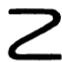
\includegraphics[keepaspectratio]{images/part001_ec6127c7.jpg}}

\begin{enumerate}
\def\labelenumi{\arabic{enumi})}
\setcounter{enumi}{1}
\item
  设 \(\mathbf{F}\) 是一个局部凸空间，它是一个递增向量子空间序列 \((\mathbf{F}_n)\) 的并，且对每个指标 \(n\) ，设 \(\mathcal{T}_n\) 是在 \(\mathbf{F}_n\) 上由拓扑 \(\mathcal{T}\) （\(\mathbf{F}\) 的）诱导的拓扑。应当注意，一般说来 \(\mathcal{T}\) 并不是诸 \(\mathcal{T}_n\) 的归纳极限。
\item
  假设 \(\mathbf{E}\) 是序列 \((\mathbf{E}_n)\) 的严格归纳极限；若 \(\mathbf{F}\) 是一个（在 \(\mathcal{T}\) 中）闭的、含于 \(\mathbf{E}\) 的向量子空间，则诸 \(\mathcal{T}_n\) 在 \(\mathrm{F} \cap \mathrm{E}_n\) 上诱导的拓扑的严格归纳极限可能严格地比 \(\mathcal{T}\) 诱导的拓扑细 (IV, 第 63 页, exerc. 10)。
\end{enumerate}

命题 10. --- 设 E, F 是两个局部凸空间。假设：

\begin{enumerate}
\def\labelenumi{\arabic{enumi})}
\item
  存在一族 Fréchet 空间 \((\mathbf{E}_{\alpha})\) ，且对每个 \(\alpha\) 有一个线性映射 \(g_{\alpha}: \mathbf{E}_{\alpha} \to \mathbf{E}\) ，使得 \(\mathbf{E}\) 的拓扑是族 \((g_{\alpha})\) 的终局部凸拓扑。
\item
  存在一个 Fréchet 空间序列 \((\mathbf{F}_n)\) ，且对每个 \(n\) 有一个连续线性单射 \(j_n: \mathbf{F}_n \to \mathbf{F}\) ，使得 \(\mathbf{F} = \bigcup j_n(\mathbf{F}_n)\) 。
\end{enumerate}

那么，每个线性映射 \(u\) （\(\mathbf{E}\) 到 \(\mathbf{F}\) 中的），只要其图在 \(\mathbf{E} \times \mathbf{F}\) 中为闭，必然连续。

为证 u 连续，只须证明对每个 \(\alpha\) ，映射 \(u \circ g_{\alpha}: E_{\alpha} \to F\) 连续 (II, 第 27 页, prop. 5)。而 \(u \circ g_{\alpha}\) 的图是 u 的图在连续映射 \(g_{\alpha} \times 1_{F}: E_{\alpha} \times F \to E \times F\) 下的逆像，因而由假设在 \(E_{\alpha} \times F\) 中是闭的。因此我们可以限于 E 本身是 Fréchet 空间的情形。但这时命题是 I, 第 20 页, prop. 1 的一个特殊情形。

推论. --- 在与 prop. 10 中关于 E 和 F 的相同假设下，并假设 E 是 Hausdorff 的，则 F 到 E 上的每个连续满射 v 是一个严格态射。

设 N 是 v 的核，并记 \(\mathrm{N}_{n}=j_{n}^{-1}(\mathrm{N})\) ；则映射 \(j_{n}^{\prime}:F_{n}/N_{n}\to F/N\) （由 \(j_{n}\) 取商得到）是单射且连续，又 \(F_{n}/N_{n}\) 是一个 Fréchet 空间（因为 \(N_{n}\) 是闭的），且 F/N 是诸 \(j_{n}^{\prime}\) 的像的并。由假设，在典范分解 \(v:F\to F/N\stackrel{w}{\to}E\) 中，线性映射 w 是双射且连续，因而其图在 \((\mathrm{F/N})\times\mathrm{E}\) 中是闭的 (GT, I, §8.1, prop. 2 的 cor. 2)。由开头的注记及 prop. 10，w 的逆映射 u 因此连续，推论得证。

* prop. 10 及其推论特别适用于如下情形：E 是一个完备的有界型空间 (III, 第 12 页)，而 F 是一个 Fréchet 空间序列的归纳极限。*

